\documentclass{article}

\usepackage{graphicx}
\usepackage{verbatim}
\usepackage{amsmath}
\usepackage{amssymb}
\usepackage[french]{babel}
\usepackage[T1]{fontenc}
\usepackage[utf8]{inputenc}
\usepackage{hyperref}
\usepackage{float}
\usepackage{listings}

%%%%%%%%%%%%%%%% Lengths %%%%%%%%%%%%%%%%
\setlength{\textwidth}{17cm}
\setlength{\evensidemargin}{0cm}
\setlength{\oddsidemargin}{0cm}

\begin{document}

\begin{titlepage}
    \centering

    
\includegraphics[width=0.25\textwidth]{logo.jpg}\par\vspace{1cm}

    {\scshape\LARGE Bordeaux INP \par}
    \vspace{0.5cm}
    {\scshape\Large ENSEIRB-MATMECA \par}

    \vspace{2.5cm}

    {\huge\bfseries Projet Robozzle \par}

    \vspace{1cm}

    {\Large Projet de programmation fonctionnelle : développement d’un jeu de programmation de robots \par}

    \vspace{3cm}

    \begin{flushleft}
        \large
        \textbf{Auteur :} VARGAS Ilan, HSSASSA Mohsine, DASSOULI Youssef\\[0.3cm]
        \textbf{Formation :} Informatique\\[0.3cm]
        \textbf{Année universitaire :} 2025--2026\\[0.3cm]
        \textbf{Encadrant :} LOMBARDY Sylvain
    \end{flushleft}

    \vfill

    {\large \today \par}

\end{titlepage}

\section*{Introduction}

Ce projet s'inscrit dans le cadre de l'unité d'enseignement de programmation fonctionnelle de sixième semestre. Il nous a été proposé de concevoir et d'implémenter un programme TypeScript permettant de faire jouer des parties, de décrire des programmes pilotant un robot, et d'en évaluer l'exécution, en prenant comme base le jeu Robozzle.

Robozzle est un puzzle de programmation dans lequel le joueur doit guider un robot sur un plateau de cases colorées afin de collecter des étoiles, en écrivant un programme composé de fonctions récursives et d'instructions conditionnelles. La contrainte centrale du jeu est son minimalisme : pas de variables, pas de boucles explicites, uniquement de la récursivité.

Ce cadre soulève une question de conception fondamentale : comment représenter un système dynamique, comme un robot évoluant dans un monde, en respectant les principes de la programmation fonctionnelle, c'est-à-dire sans état mutable et par composition de types abstraits ?

C'est autour de cette problématique que s'organise ce rapport, en suivant la hiérarchie de modules construite au cours du développement : des types fondateurs jusqu'à l'évaluateur et l'interface interactive.

\tableofcontents

\section{Architecture}

L'architecture de Robozzle repose sur un principe de composition modulaire ascendante, inspiré des paradigmes de la programmation fonctionnelle. Chaque composant est construit à partir des éléments définis précédemment, formant une hiérarchie de concepts de complexité croissante.

\begin{figure}[h]
    \centering
    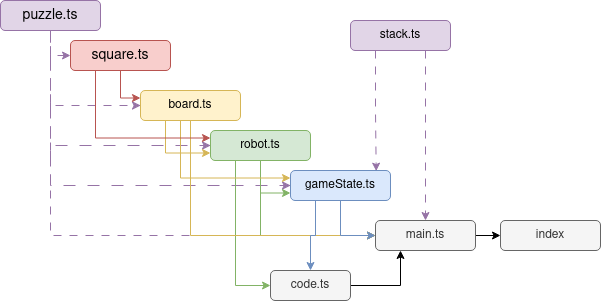
\includegraphics[width=0.6\textwidth]{archi_robot.png}
    \caption{Architecture du projet Robozzle}
    \label{fig:archi}
\end{figure}

Comme illustré par la figure \ref{fig:archi}, l’architecture repose à sa base sur le modules \textit{puzzle.ts}, qui contient des définitions de types et d’énumérations structurant le reste du code, et \textit{stack.ts}, chargé de l’implémentation de la pile.

Nous définissons le type de base \textit{Square} dans \textit{square.ts} représentant la cellule élémentaire de la grille de jeu. \`A partir de ce type , nous définissons le type abstrait \textit{Board}, un assemblage de squares de manière à former la grille de jeu, et puis \textit{Robot} qui est composé d’une position (définit par \textit{Square}) et une direction pour représenter un agent qui manipule un board.

Dans \textit{gameState.ts}, à partir de \textit{Board}, \textit{Robot} et \textit{Stack}, nous définissons l’état de jeu \textit{State}, capable de décrire de manière indépendante un jeu et son avancement, et une \textit{Action} qui modifie un \textit{State} en un autre faisant ainsi avancer la partie.

Finalement, avec les états de jeu, nous pouvons définir une interface de jeu via une couche graphique.

Cette approche reflète un principe fondamental de la programmation fonctionnelle : construire des abstractions complexes par composition de types simples sans recourir aux l'état mutable. Chaque module est autonome, testable isolément, et ne dépend que des couches inférieures. 
\\

Pour chaque couche, nous utilisons les types définis dans les couches inférieures comme briques de construction. \textit{Board} est construit à partir de \textit{Square}, \textit{Robot} à partir de \textit{Square} et \textit{Dir}, \textit{State} à partir de \textit{Board}, \textit{Robot} et \textit{Stack}. Chaque nouveau type abstrait enrichit les précédents sans les modifier, en les composant pour former une abstraction de niveau supérieur. C'est ce principe de composition ascendante qui donne à l'architecture sa cohérence : on ne repart jamais de zéro, on s'appuie sur ce qui est déjà défini et testé.

Nous remarquons dans la figure \ref{fig:archi} que plus les modules sont dans les couches externes au sens de dépendances et plus il dépendent d'un plus gros nombre de couches internes. Cela est visible principalement aux modules d'entrée au programme comme \textit{code.t} ou \textit{main.ts} qui doivent gérer tous ces modules.


\section{Les types de base}

L’architecture de notre projet est définie par des types fondamentaux utilisés par les modules qui suivent permettant de mieux ce communiquer entre eux et construire au dessus de ces types pour former des plus complexes.

\subsection{Fichier partagé puzzle}

Le fichier \textit{puzzle.ts} prend le rôle d’un fichier de déclarations contenant un ensemble de constantes globales et types basiques qui servent de vocabulaire commun entre les modules.

Nous y définissons la taille du plateau de jeu, les énumérations \textit{Dir} et \textit{Color} encodant respectivement les direction cardinales et couleurs des cases, le type \textit{Pos} position $x,y$, ainsi que le type \textit{Puzzle} qui reflète fidèlement la structure JSON reçue en entrée. Ce fichier sert de base sur lequel s'appuient tous les autres modules. 

\subsection{Introduction de stack}

Le module \textit{stack.ts} définit un type abstrait générique \textit{Stack<T>}, paramétré par le type des éléments qu'il contient. 

La pile est implémentée comme une liste chaînée immuable avec une sentinelle à la fin : toute opération produit une nouvelle pile sans modifier l'existante, conformément aux principes de la programmation fonctionnelle. Le module expose les opérations classiques \textbf{cons, head, tail, stackIsEmpty}.

Nous attribuons également un attribut spéciale \texttt{nb} qui contera le nombre de calls, cela sera utile pour \textit{State} et aborderons postérieurement.

\subsection{Type de base square}

Le module \textit{square.ts} définit le premier type abstrait du projet : \textit{Square}. Un square est caractérisée par sa couleur \texttt{.color}, sa position pos \texttt{.position} sur le plateau et la présence éventuelle d'une étoile \texttt{.isStar}. 

Le module expose également une valeur sentinelle \texttt{out}, représentant l'extérieur du plateau ou une case vide, ainsi que l'opération \textbf{squareIsOut} permettant de tester ce cas limite, \texttt{squareIsOut(square) === true} si \texttt{square} est \texttt{out}. Par la suite, pour représenter la position non valide \textit{fell out of board}, nous utiliserons \texttt{out}.

Square est le type fondateur de la hiérarchie, c'est à partir de lui que le plateau est construit et, avec le plateau constitué de squares uniques, un square représente un position.


\section{Type abstrait Board}

\subsection{Définition}

Le module \textit{board.ts} définit le type abstrait \textit{Board}, qui représente l'état du plateau de jeu. Un \textit{Board} est composé d'un tableau \texttt{.board} de squares, enrichi de deux informations supplémentaires : la case de départ du robot \texttt{.start} pointeur vers un square et le nombre d'étoiles restantes \texttt{.nbStars}. Ce dernier permet de déterminer la condition de victoire sans avoir à parcourir le plateau entier.

Le tableau \texttt{board} est lu comme une matrice de squares avec en sachant la largeur du tableau : $i * puzzle_{width} + j = k$ avec $k$ l’indice dans .board. On a ainsi une représentation de matrice de squares donc un plateau.

\subsection{Méthodes}

La fonction \textbf{boardInit} assure la conversion d'un puzzle brut en un board exploitable. Cette conversion repose sur deux fonctions récursives internes.
\begin{itemize}
	\item \textbf{boardMap} qui parcours la chaîne de caractères Puzzle.board et renvoie un tableau de \textit{Square} qui associe pour chaque caractère un square. On se base sur \texttt{.map()} javascript mais pour une chaîne de caractère, on passe en argument la fonction qui crée un \textit{Square} associé à un caractère. C’est avec cette fonction qu’on crée le .board;
	\item \textbf{boardFold} basé sur \texttt{.reduce()} pour une chaîne de caractères, on utilise la fonction qui compte +1 au accumulateur si la lettre est majuscule, représentant une case avec une étoile. On l'utilise pour calculer \texttt{nbStars}.
\end{itemize}

La fonction \textbf{removeStar} enlève l’étoile d’un square donné dans un board donné. La subtilité avec la programmation fonctionnelle est que pour changer l’état d’une variable nous devons créer une nouvelle, ainsi pour enlever l’étoile d’un square $s$ d’un board $b$, nous commençons par créer un nouveaux square $s'$ avec les mêmes attributs que $s$ à l'exeption de $s.isStar$ qui devient $false$. Puis nous créons un nouveau board $b'$ tel que $b'$.board est le tableau contenant tous les anciens squares de $b$ sauf $s$ substitué par $s'$. Finalement $nbStars_{b’} = nbStars_{b} - 1$.

Nous avons une compléxité mémoire de la taille d'un square et d'une structure board (avec .board un pointeur de \textit{Square}) 
\\

Le module expose également deux opérations fondamentales : \textbf{isWin}, qui teste si la partie est gagnée ($.nbStars = 0$) et \textbf{move2square}, qui renvoie la case voisine dans une direction donnée d’un square dans un board.


\section{Robot et actions sur Game}

Le module \textit{robot.ts} définit le type abstrait \textit{Robot} et l'encapsulation \textit{Game} qui permet de faire des actions sur un robot.

\subsection{Définition de Robot}

Le type \textit{Robot} est définie par une position \texttt{.square} représenté par un \textit{Square}, dont nous avons déjà établit que cela représente une position, et une \texttt{.dir} direction \textit{Dir}.

On notera également l'utilisation de \texttt{generalSquare}, une fonction d'ordre supérieur générique qui factorise l'accès aux attributs du Square sous-jacent au robot.

\subsection{Encapsulateur Game et actions game}

Nous encapsulons un robot et un board dans un type \textit{Game}. Nous pouvons faire des actions sur \textit{Game}, c’est-à-dire des fonctions qui prennent un game et retournent un autre.

 Nous définissons ainsi \textbf{turnRight, turnLeft} qui tournent robot de game, c’est-à-dire modifie la direction du robot horaire ou antihoraire, et \textbf{moveForward} qui fait avancer le robot dans le board, donc change .square en créant un nouveau robot qui sera retourné par la fonction.

Board doit être inclus en argument et retourné car l’action peut le changer, par exemple \texttt{gameNew = moveForward(game)} peut avoir le robot sur un square étoile ce qui signifie qu’il faut créer un nouveau bord sans cette étoile. Si board n'est pas modifier alors on retourne lui même.

C’est la responsabilité de l’action de vérifier ces cas (\texttt{square.isStar === 1} pour l'exemple précédent) mais c’est à \textit{board.ts} de manipuler le board (move2square pour bouger robot, removeStar pour un nouveau board sans l’étoile). 


\subsection{Observations sur l’abstraction et découplage}

C'est ici que l'on peut constater le bénéfice de notre architecture. \textit{Square} aurait pu être une simple paire de coordonnées (x, y) dans une matrice dans \textit{Board}, un pointeur vers un élément du tableau dans \textit{Board} ou encore un sommet de graphe représenté par \textit{Board} comme envisagé initialement. Du moment que \textit{Square} expose les attributs \texttt{isStar} et \texttt{color} ainsi que ses méthodes, le module de \textit{robot.ts} fonctionne. L'abstraction introduite par \textit{square.ts} découple \textit{robot.ts} de toute décision d'implémentation prise dans \textit{board.ts} et \textit{square.ts}.

Nous continuerons dans cette logique en construisant chaque nouveau type abstrait à partir des précédents. Chaque couche enrichit la précédente en ajoutant un niveau d'abstraction supplémentaire, sans jamais en exposer les détails internes. Cette composition ascendante de TADs est le principe structurant de l'ensemble du projet.


\section{Tests et validité}

Les tests ont été écrits avec Jest et couvrent les trois modules fondateurs : \textit{stack.ts}, \textit{square.ts} et \textit{board.ts}. Ils constituent un outil de vérification du comportement attendu de chaque TAD, mais aussi un filet de sécurité contre les régressions lors des modifications du code.
\\

Chaque suite de tests est organisée par opération. Pour chaque fonction exposée, on teste le cas nominal, les cas limites, et les invariants importants. Par exemple :
\begin{itemize}
  \item vérifier qu’une pile vide est uniquement représentée par \texttt{nil} ;
  \item garantir que \texttt{cons} ne modifie pas l’attribut \texttt{nb} ;
  \item tester les déplacements hors du plateau ;
  \item vérifier la suppression correcte d’une étoile et la mise à jour cohérente de \texttt{nbStars} ;
  \item valider la détection des dépassements de pile avec \texttt{isOverStack}.
\end{itemize}

Une attention particulière a été portée aux propriétés d’immuabilité. Plusieurs tests vérifient explicitement que les anciennes structures restent inchangées après création d’une nouvelle version, ce qui est essentiel dans notre architecture fonctionnelle.
\\

L’utilisation de Jest et de son outil de couverture a permis d’évaluer quantitativement les tests réalisés. Les résultats obtenus montrent une couverture de :
\begin{itemize}
\item 97.43\% des instructions ;
\item 85.71\% des branches ;
\item 100\% des fonctions ;
\item 96.96\% des lignes.
\end{itemize}

Les 31 tests passent, avec une couverture globale de 97,43\% des instructions et 100\% des fonctions jusqu’à présent. Les deux lignes non couvertes dans board.ts (lignes 41 et 84) correspondent au cas default des switch sur les directions et les couleurs, des branches défensivement écrites mais inatteignables avec les types actuels.

La couverture de branches s'établit à 85,71\%, écart principalement dû à ces mêmes cas default. 
\\

Chaque type abstrait de données possède sa propre suite de tests dédiée. Cette séparation suit directement l’architecture modulaire du projet : chaque couche est validée indépendamment avant d’être utilisée par les couches supérieures. Ainsi, les tests de \textit{stack.ts} garantissent les propriétés fondamentales de la pile immuable, sur lesquelles reposent ensuite les modules \textit{gameState.ts} et \textit{main.ts}.


\section{Module GameState}

Le module \textit{gameState.ts} constitue le sommet de la hiérarchie de composition. Il définit le type \textit{State}, qui représente l'état complet du jeu à un instant donné et introduit la notion de \textit{Action} qui permettra de passer d’un state à un autre.

\subsection{Définitions}

Un \textit{State} est composé d’un board, un robot et une pile d’action \textit{Stack<Action>}, \texttt{.stack}, à exécuter. Cela représente de manière indépendante un jeu complet en un moment donné.

Un state seul est un état de jeu à un moment donnée, pour cela nous définissons une \textit{Action} qui est une fonction qui prend en argument un state et retourne nouveau state, soit une fonction de transition. C'est similaire à action game mais pour tout le \textit{State} inclut le .stack. Le passage de un state à un autre par une action est un pas. 

Nous définissons également une \textit{Function} qui est un tableau d'action. Le joueur donnera un tableau de functions \texttt{arrayFunct} en début de partie selon les spécifications du puzzle.

Les actions permettent d’avancer, au sens de pas, dans la partie de state en state, et sont contenues dans la pile .stack. L’idée est de construire state initiale avec avec un stack remplies des actions de la fonction initiale de \texttt{listFunc}, chaque tour on dépile la première action de .stack, on applique au state lui même ce qui nous donne un nouveau state donc on répétera le même processus de manière récursive jusqu’à ne plus avoir d’actions (on peut plus avancer) ou atteindre une autre condition de base de fin de partie. La fonction qui applique head stack action à state est \textbf{popStack} : \texttt{newState = popStatck(state)}.

En conclusion, un state définit un état et décrit ses prochains récursivement.

\subsection{Constructeur d’action}

Il y a deux types d’actions : des \textit{actions on game} ou des \textit{action call}.
\\

Une \textit{actions on game} est simplement une action game définit précédemment dont on dépile l’action concernée du stack pour ne pas la répéter.

\begin{figure}[H]
    \centering
    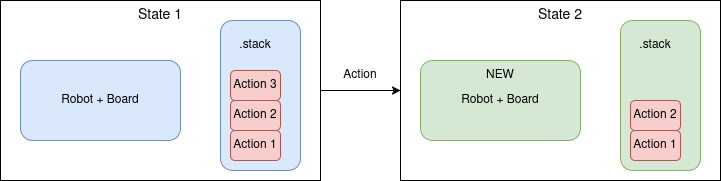
\includegraphics[width=0.8\textwidth]{action_game.png}
    \caption{Illustration d'un game based action}
    \label{fig:action_game}
\end{figure}

Pour écrire cette action nous définissons le constructeur \textbf{actionGame} qui convertit un action game (turn, move forward) en une action, c’est-à-dire additionne le dépilement du stack. Nous pouvons ajouter une condition aussi sur robot, si elle est fausse, on dépilera sans faire action game.
\\

Un \textit{action call} est une action qui dépile l'action (pour pas répéter) et empile les actions de function dans le bon ordre.

\begin{figure}[H]
    \centering
    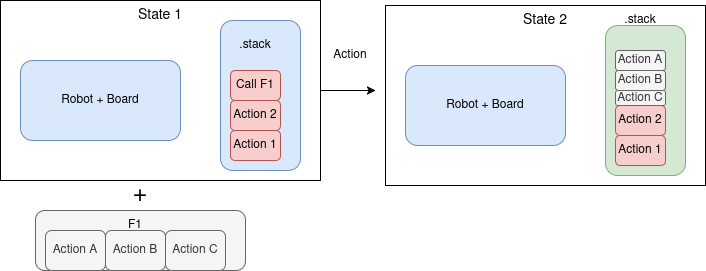
\includegraphics[width=0.8\textwidth]{action_call.png}
    \caption{Illustration d'un call action}
    \label{fig:action_call}
\end{figure}

Nous définissons le constructeur \textbf{actionFunct} qui convertit un function en action en dépilant le call et en empilant tous les action en appliquant \texttt{.reduce((acc: Stack<Action>, curr: Action) => cons(curr, acc), stackCall)} à function, c'est-à-dire on applique un algorithme \textit{folder} avec une fonction qui concatène avec l'action current au stack accumulateur, avec pour stack initial le stack dont action call à été dépilé (et un call stack expliqué plus tard).

Remarquez que l’ordre des actions sur la pile. Comme illustré par la figure \ref{fig:action_call}, on veut avoir l’action A en head par la logique de récursivité et call stack, or il serait en $3^{eme}$ position en empilant normalement. Pour cela nous créons une copie de function avec l'ordre des actions inversés avant d'appliquer le folder.

\subsection{Conditions de fin de partie}

Les condition de fin de partie sont le stack être vide \texttt{istackIsEmpty(aState.stack)}, avoir gagné \texttt{isWin(aState.board)}, l’agent être tombé \texttt{robotIsFell(aState.robot)} ou avoir un \textit{overstack} \texttt{isOverStack(aState.stack)}.

Cette dernière condition mérite une attention particulière. Robozzle autorise les fonctions récursives : une fonction peut s'appeler elle-même indéfiniment, provoquant une croissance infinie de la pile d'exécution. Pour détecter ce cas, le type \textit{Stack<T>} maintient un attribut \texttt{nb} qui comptabilise le nombre d'appels de fonctions effectués. Cet attribut est incrémenté exclusivement par l'opération \textbf{call(action, Stack<Action>)}, méthode similaire à \texttt{cons} mais tel que \texttt{call(action, stack).nb = stack.nb + 1}, contrairement \texttt{cons(action, stack).nb = stack.nb}.

\texttt{call} est utilisée dans \texttt{actionFunct} pour le premier empilement avant \texttt{.reduce(...)}. Lorsque \texttt{nb} dépasse 50, \textbf{isOverStack} est vérifiée et la partie se termine. Ce mécanisme permet d’interrompre toute exécution divergente.

\begin{figure}[H]
    \centering
    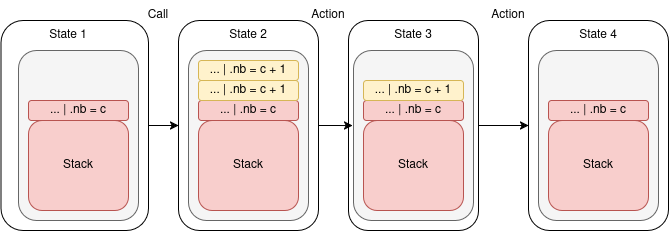
\includegraphics[width=0.6\textwidth]{nb_call.png}
    \caption{Illustration de l'attribut .nb dans un call}
    \label{fig:nb_call}
\end{figure}

\`A noter que quand toutes les actions liées à un call sont dépiler alors stack.nb reviens à .nb d’avant car les stacks ne sont pas modifiables comme illustré par la figure \ref{fig:nb_call}.

En combinant tout, nous avons:

\begin{figure}[H]
\centering
\begin{lstlisting}[language=, basicstyle=\ttfamily\small, frame=single, breaklines=true, captionpos=b]
function actionFunct(aFunctTrunk: () => Funct, cond?: (g: Robot) => boolean): Action {
  return (aState: State) => {
    // creation d'une fonction d'action d'ordre inversee
    const aFunct = aFunctTrunk().slice().reverse();
    // Si condition en robot vrai alors faire call
    if (cond === undefined || cond(aState.robot)) {
      
      // Fonction pour marquer call en stack
      // Avant d'appeller on depile action call
      const stackCall =
        (aFunct.length > 0)
          ? call(aFunct[0], tail(aState.stack))
          : tail(aState.stack);

      // Creation d'un nouveau tableau en empilant toutes 
      // action de function dans call       
      const stackNew = aFunct.
        slice(1).
        reduce((acc: Stack<Action>, curr: Action) => cons(curr, acc), 
               stackCall);

      // Retourner nouvel state
      return {
        robot: aState.robot,
        board: aState.board,
        stack: stackNew
      };
    } else {
      // Sinon on depile action call
      return {
        robot: aState.robot,
        board: aState.board,
        stack: tail(aState.stack)
      };
    }
  };
\end{lstlisting}
\caption{Algorithme du constructeur \texttt{actionFunct}}
\label{code:action_call_cons}
\end{figure}

Il y a une chose qu'on a pas expliqué, c'est a troncatrure \texttt{aFunctTrunk: () => Funct} dont nous allons expliquer dans la prochaine partie.



\section{Le langage et l'évaluateur}

La prochaine étape naturelle consiste à concevoir un langage simplifié permettant de décrire des programmes pilotant un robot. 

\subsection{Conception du langage}

Robozzle repose sur un modèle de programmation par fonctions : un programme est un ensemble de fonctions numérotées, chacune étant une séquence d'instructions élémentaires. 

Les instructions disponibles sont les mouvements du robot, les rotations, et les appels de fonctions. Chaque instruction peut être conditionnée par la couleur de la case sur laquelle se trouve le robot. C’est un modèle minimaliste sans variables ni boucles explicites, le seul mécanisme de répétition est la récursivité. C'est à partir de cette spécification que nous avons élaboré notre langage en TypeScript.

Dans notre implémentation, ce langage repose sur deux concepts fondamentaux : les \textit{Action} et les \textit{Funct}.

Une \textit{Action} constitue l’instruction élémentaire du langage. Elle se décline sous deux formes :
\begin{itemize}
    \item les \textit{actionGame}, qui correspondent aux actions exécutées sur le robot (\textit{moveForward}, \textit{turnLeft}, \textit{turnRight}) ;
    \item les \textit{actionCall}, qui permettent l’appel d’une fonction.
\end{itemize}

Ces actions peuvent être associées à une condition optionnelle par rapport à l’état du robot ou la couleur de la case courante. 

Une \textit{Funct} est alors définie comme une séquence ordonnée d’actions. Un programme complet est composé de cinq fonctions, chacune contenant un nombre fini d’actions selon les contraintes du puzzle courant. Certaines fonctions peuvent, ou même doivent, être vides. L'ensemble des cinq \textit{Funct} constitue le programme complet, rassemblé le tableau \texttt{arrayFunct}. C'est l'unique point d'entrée mis à disposition du joueur pour écrire son programme.

Finalement le joueur peut décider l’id du puzzle en modifiant \texttt{puzzle\_id}. Tout cela se trouve dans le fichier \textit{code.ts}, le seul fichier que le client à le droit de modifier.

\subsection{Évaluateur}

L'évaluateur est le mécanisme qui, étant donné un programme et un monde initial, réalise l'exécution pas à pas et produit un résultat. Il repose sur trois fonctions fondamentales.

\subsubsection{Initialisation}

La fonction \texttt{initState} construit l'état initial à partir du puzzle et du programme fourni par le joueur. 

Le robot est positionné sur la case de départ avec la direction indiquée par le puzzle. La pile d'exécution est initialisée avec les actions de \texttt{arrayFunct[0]}, la première fonction constitue le point d'entrée du programme. La function est reversed puis réduites en pile via \texttt{cons}, de sorte que la première action de la fonction se retrouve en tête de pile. Le board est initialisé par \texttt{boardInit} avec comme argument le puzzle.

\subsubsection{Pas d'exécution}

La fonction \texttt{popStateStack} constitue le cœur de l'évaluateur. Il prend un state en paramètre, prend l'action head de la stack et applique au state produisant un nouveau state. Ce processus est purement fonctionnel : aucun state n'est modifié en place.

\subsubsection{Condition de fin et résultat}

La fonction \texttt{isEnd} détermine si l'exécution doit s'arrêter. On distingue deux cas :
\begin{itemize} 
\item Victoire si toutes les étoiles ont été ramassées, (\texttt{isWin});
\item Défaire si la pile est vide (\texttt{stackIsEmpty}), si le robot est tombé du plateau (\texttt{robotIsFell}) ou nombre d’appelle au dessu de l’autorité (\texttt{isOverStack}). 
\end{itemize}

\subsection{Exemple concret}

Le fichier code.ts illustre concrètement l'écriture d'un programme pour le puzzle 330 :

\begin{figure}[H]
\centering
\begin{lstlisting}[language=, basicstyle=\ttfamily\small, frame=single, breaklines=true, captionpos=b]
const puzzle\_id = 330;

const arrayFunct: Array<Funct> = [[
    actionFunct(() => arrayFunct[1]),
    actionGame(turnRight),
    actionGame(moveForward)
  ],
  [
    actionGame(moveForward),
    actionGame(turnRight, (r) => robotColor(r) === Color.RED),
    actionFunct(() => arrayFunct[1], (r) => robotColor(r) === Color.BLUE),
    actionGame(moveForward)
  ],
  [], [], []
];
\end{lstlisting}
\caption{Exemple de codage}
\label{code:code}
\end{figure}

La fonction 0 est le point d'entrée : elle appelle la fonction 1, tourne à droite, puis avance. La fonction 1 avance, tourne à droite si la case est rouge, s'appelle récursivement si la case est bleue, puis avance. On voit ici la récursivité \texttt{actionFunct(() => arrayFunct[1])} rendue possible par l'utilisation d'un thunk \texttt{(() => arrayfunct[1])} pour éviter la référence au moment de l'initialisation, sinon nous référençons à arrayfunct[1] depuis arrayfunct[0], un tableau non encore initialisé. 
\\

Pour construire les actions, nous utilisons les constructeurs présentés précédemment. 
\begin{itemize}
  \item Si nous voulons faire un call :  \texttt{actionFunct(() => arrayFunct[\textit{numéro de fonction}], \textit{condition optionnel})};
  \item Si nous voulons faire une action sur le robot : \texttt{actionGame(\textit{action de game}, \textit{condition optionnel})};
\end{itemize}




\section{Main et interface graphique}

L'objectif dans cette partie est de créer une interface interactive entre le joueur et le système. Nous voulons que le joueur puisse avancer ou reculer au sens de l’évaluation entre les states comme il le souhaite.

\subsubsection{Couche principale}

Le fichier \textit{main.ts} est une interface entre notre évaluateur et la couche graphique. Nous implémentons les fonctions qui permettent cette navigation entre les state.

Pour cela nous implémentons la seule variable mutable du programme : \texttt{stateStack}. Il s’agit d’une pile de \textit{State} qui maintient l’historique de states. Il est important ici qu'elle soit mutable car les fonctions à suivre modifient l'historique à chaque interaction, et cette pile doit être dans une addresse global constante pour être référencé par les fonctions à suivre. 

\`A l’état initiale, \texttt{stateStack} est la pile contenant seulement le initial state et, à tout moment, head de \texttt{stateStack} est le state courant : les states s’empile gardant le plus récent au-dessus.

Trois fonction manipulent \texttt{stateStack}:
\begin{itemize} 
\item \texttt{step} : avance d'un pas en appliquant \texttt{popStateStack} au head de \texttt{stateStack} et empile le nouvel état sur \texttt{stateStack}, on doit vérifier d’abord que on est pas dans un state finale pour l'utliser; 
\item \texttt{back} : recule d'un pas en dépilant \texttt{stateStack} et renvoyant head, attention car si \texttt{stateStack} est vide alors on peut plus rien faire ainsi, par sécurité, si nous somme dans l’état initiale nous renvoyons head sans dépiler; 
\item \texttt{restart} : reinitialise \texttt{stateStack} à l'état initial. 
\end{itemize}

La fonction \texttt{stateToUI} assure la conversion d'un \textit{State} en \textit{StateUI}, une représentation simplifiée destinée à l'afficheur. Cette couche de séparation garantit que la logique du jeu reste indépendante de toute décision d'affichage..

\subsubsection{Afficheur}

L'afficheur reçoit des \textit{StateUI} et met à jour le DOM en conséquence. Le plateau est rendu sous forme de tableau HTML, chaque case portant une classe CSS selon sa couleur. Le robot est représenté par une police d'icônes personnalisée (\texttt{robots.ttf}), définissant seize glyphes dont quatre orientations du robot et une étoile.

Quatre boutons permettent l'interaction : 
\begin{itemize}
  \item \textit{step} pour avancer : on appelle \texttt{step} en verifiant \texttt{!isEnd}, recevons un \textit{StateUI} puis actualisons le DOM;
  \item \textit{back} pour reculer : on appelle \texttt{back} et actualisons;
  \item \textit{play} pour exécuter automatiquement pas à pas avec un délai de 100ms jusqu’à arriver dans un state finale;
  \item \textit{restart} pour réinitialiser. L'afficheur délègue entièrement la logique à \texttt{main.ts} et ne manipule que la présentation.
\end{itemize}

\begin{figure}[H]
    \centering
    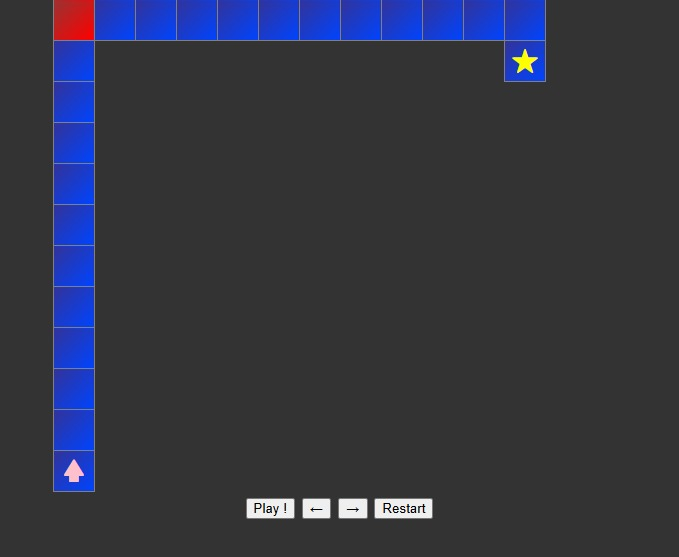
\includegraphics[width=0.6\textwidth]{interface.jpeg}
    \caption{Interface graphique projet robozzle}
    \label{fig:ui}
\end{figure}



\section*{Conclusion}

Ce projet nous a permis de mettre en pratique les principes fondamentaux de la programmation fonctionnelle dans un contexte concret et complet : de la définition des types de base jusqu'à l'interface interactive, en passant par l'évaluateur.

Le fil directeur de l'ensemble du développement est la composition de types abstraits. Plutôt que de construire un système monolithique, nous avons décomposé le problème en modules autonomes, chacun définissant un TAD à partir des couches inférieures. Cette approche a naturellement produit un code modulaire, testable isolément, et robuste aux changements d'implémentation. L'immuabilité, appliquée systématiquement, a simplifié le raisonnement sur le comportement du programme et rendu possible des fonctionnalités comme le retour en arrière sans complexité supplémentaire.

Ce projet illustre ainsi comment les paradigmes de la programmation fonctionnelle tels que l’abstraction, la composition, l’immuabilité, ne sont pas de simples contraintes théoriques, mais des outils concrets qui guident la conception vers des architectures plus claires et plus maintenables.

Parmi les fonctionnalités proposées par le sujet que nous n'avons pas implémentées figurent la génération automatique de puzzles et la recherche de solutions, qui constituent des prolongements naturels s'appuyant directement sur l'évaluateur existant.

\end{document}
